\section{Integration}
\label{sec:integration}

\subsection{Client Side}
\label{subsec:Client Side}
The Captcha service integrates seamlessly into existing web applications. It basically works by appending an invisible overlay to the body element of the existing website. The overlay fades in when the user hits the submit button of the captcha protected form. Thereby it does not affect the layout of the existing websites.
\begin{figure}[H]
	\centering
	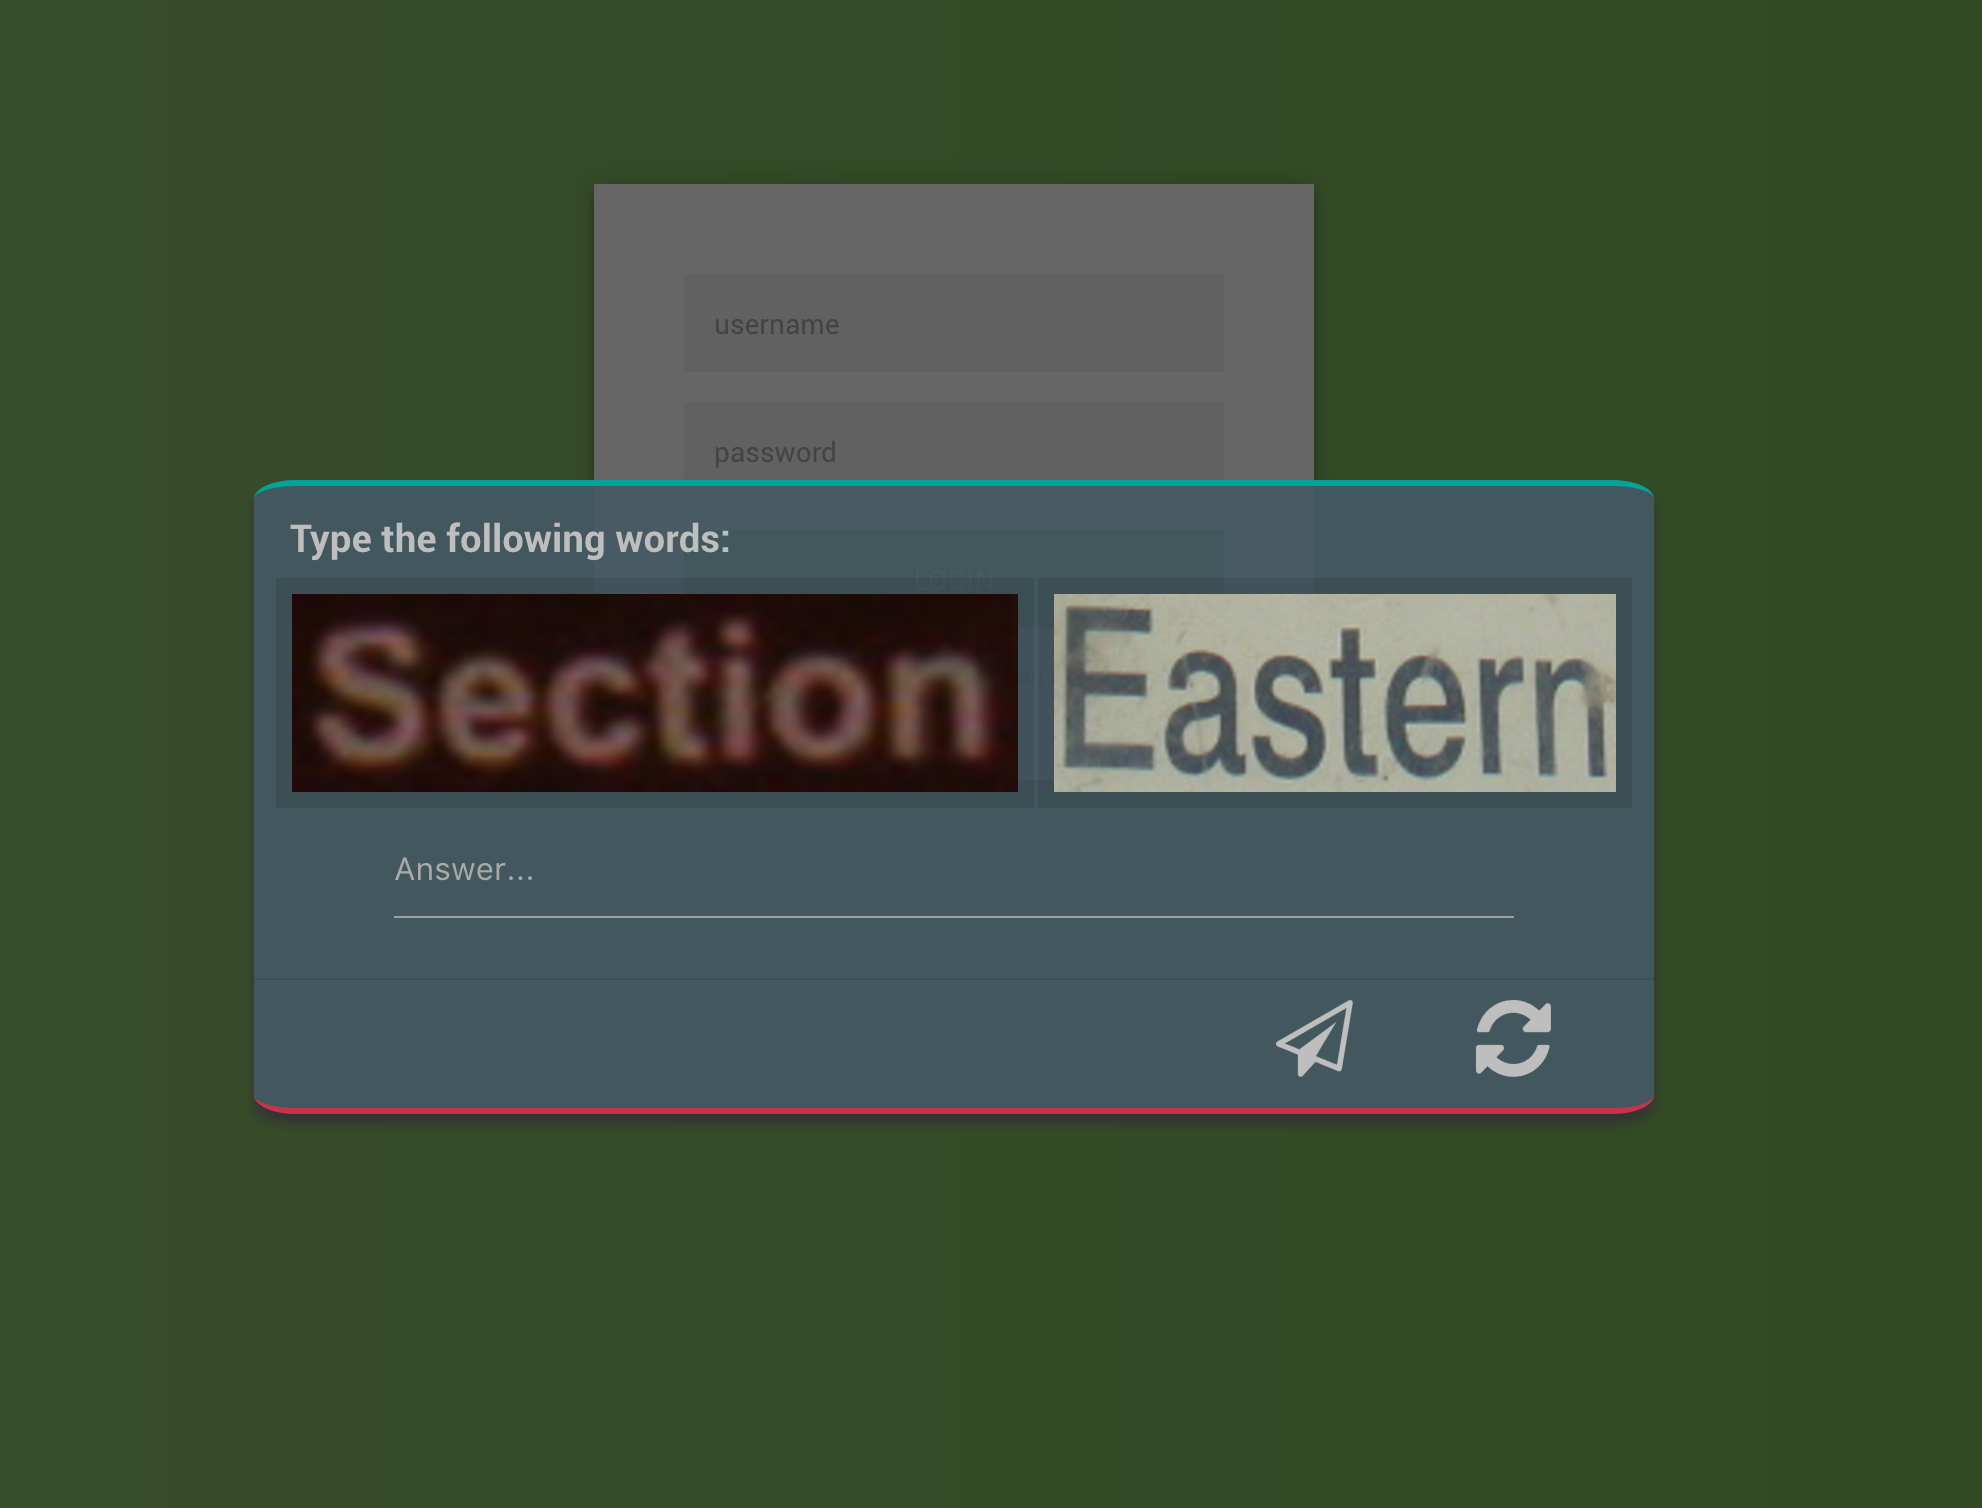
\includegraphics[width=0.8\linewidth]{content/figures/captcha_words.png}
	\caption{Captcha card contents}
	\label{fig:captcha_words}
\end{figure}

 The overlay consists of a \textit{Captcha card}, which in turn consists of a \textit{task}, to be solved \textit{Captcha tokens} and \textit{submit} and \textit{refresh} action elements, as shown in fig. \ref{fig:captcha_words}. As mentioned earlier, we currently support two different Captcha types - namely \textit{text} and \textit{image captchas} - which are randomly delivered to the client. 
 
 \begin{figure}[H]
	\centering
	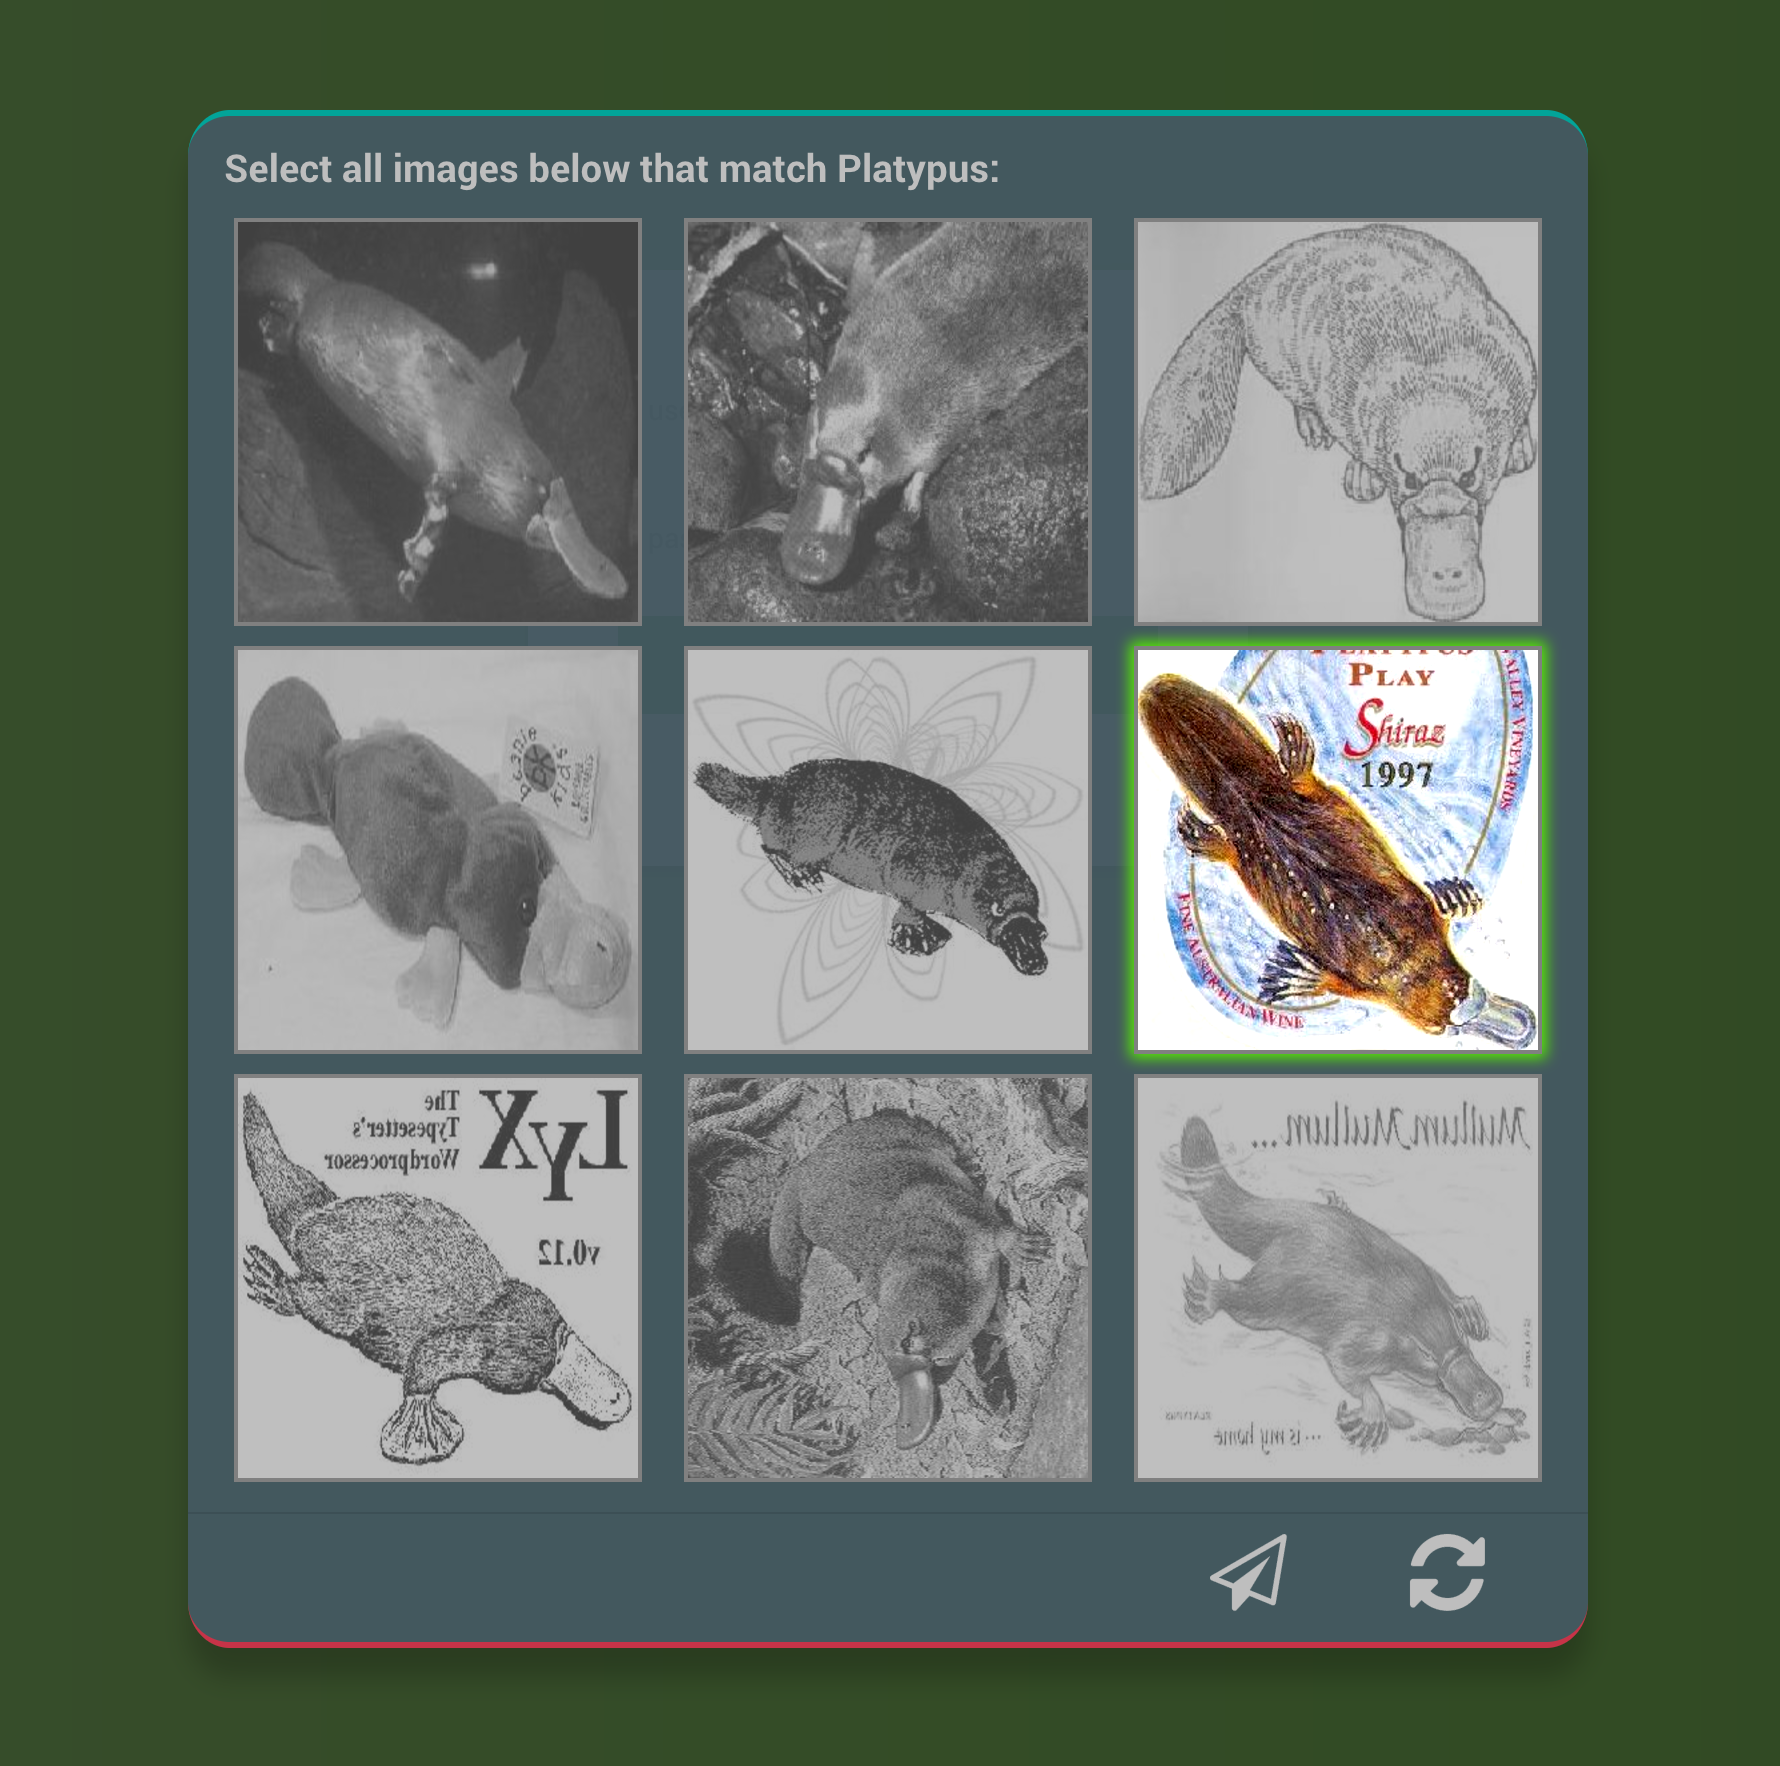
\includegraphics[width=0.8\linewidth]{content/figures/captcha_images.png}
	\caption{Image captcha session}
	\label{fig:captcha_images}
\end{figure}
 
 As soon as the user visits the page, the browser opens a session at the Captcha service via REST API. The browser receives a \textit{session key}, the \textit{Captcha type}, a list of \textit{Captcha tokens} and - in case of an \textit{image Captcha session} - a \textit{task}. The \textit{session key} gets stored in a hidden input field in the Captcha protected form. As a result the \textit{session key} is sent to the web application as soon as the form is submitted, in order to make sure that the client properly solved the Captcha at a later point in time. 
 
 Determined by the \textit{Captcha type} the \textit{Captcha tokens} get either rendered as \textit{text Captcha tokens}, as shown in fig. \ref{fig:captcha_words}, or as \textit{image Captcha grid}, as depicted in fig.\ref{fig:captcha_images}. In case the \textit{session type} is an \textit{image Captcha session}, the task is generated dynamically by inserting the delivered \textit{task} into the HTML, unlike the text Captcha task, which is static.
 
 When the client hits the reload button, the Captcha service is asked via REST API to renew the \textit{session's Captcha tokens}. The response consists of a new list of \textit{tokens} of the same type as before. Subsequently, the old \textit{Captcha tokens} are replaced by the freshly received \textit{Captcha tokens}. The \textit{submit action} triggers the server-side solution validation via REST API. In case the solution was correct the form gets submitted including the \textit{session key}. When the solution is incorrect, the \textit{Captcha card} shakes in order to visually indicate the wrong solution and all newly assigned \textit{Captcha tokens} are inserted. This happens in order to prevent brute force solving. As soon as a wrong solution is submitted, the Captcha service assigns new \textit{Captcha tokens} to the \textit{session} and returns them as response to the client. As a result, you can not restore the old \textit{session tokens} and try to solve it by using all possible inputs.

\subsection{Captcha Integration Workflow}
\label{subsec:Captcha Integration Workflow}

Integrating the Captcha service into your existing web application is fairly easy. You have to take the following steps:
\begin{enumerate}
	\item inject \texttt{captcha.min.css} and \texttt{captcha.min.js} to your HTML skeleton
	\item  Make sure the to be protected captcha form has the class \textit{captcha-form} and the corresponding submit button possesses the class \textit{captcha-button}
	\item Finally, integrate an additional POST request to our captcha service including the clients \textit{session key} into your existing server-side code, that receives the form data, in order to assure that the user solved the Captcha correctly and did not modify the javascript code.
\end{enumerate}

\texttt{captcha.min.js} includes the client-side code, whose behaviour is described in the last section. \texttt{captcha.min.css} provides the initial styling. Feel free to modify it, such that it fits your design. 

\clearpage
